\documentclass[onecolumn, draftclsnofoot,10pt, compsoc]{IEEEtran}
\usepackage{graphicx}
\usepackage{url}
\usepackage{caption}
\usepackage{setspace}

\usepackage{geometry}
\geometry{textheight=9.5in, textwidth=7in}

% 1. Fill in these details
\def \CapstoneTeamName{         The Cleverly Named Team}
\def \CapstoneTeamNumber{               68}
\def \GroupMemberOne{                   Tyler Jones}
\def \GroupMemberTwo{                   Avi Sinha}
\def \GroupMemberThree{                 Sam Cooney}
\def \CapstoneProjectName{              Investment Performance Mobile Application}
\def \CapstoneSponsorCompany{   HedgServe}
\def \CapstoneSponsorPerson{            Edison Tsai}

% 2. Uncomment the appropriate line below so that the document type works
\def \DocType{          %Problem Statement
                                %Requirements Document
                                %Technology Review
                                Design Document
                                %Progress Report
                                }

\newcommand{\NameSigPair}[1]{\par
\makebox[2.75in][r]{#1} \hfil   \makebox[3.25in]{\makebox[2.25in]{\hrulefill} \hfill            \makebox[.75in]{\hrulefill}}
\par\vspace{-12pt} \textit{\tiny\noindent
\makebox[2.75in]{} \hfil                \makebox[3.25in]{\makebox[2.25in][r]{Signature} \hfill  \makebox[.75in][r]{Date}}}}
% 3. If the document is not to be signed, uncomment the RENEWcommand below
%\renewcommand{\NameSigPair}[1]{#1}

%%%%%%%%%%%%%%%%%%%%%%%%%%%%%%%%%%%%%%%
\begin{document}
\begin{titlepage}
    \pagenumbering{gobble}
    \begin{singlespace}
       %\includegraphics[height=4cm]{}
        \hfill
        % 4. If you have a logo, use this includegraphics command to put it on the coversheet.
        %\includegraphics[height=4cm]{CompanyLogo}
        \par\vspace{.2in}
        \centering
        \scshape{
            \huge CS Capstone \DocType \par
            {\large\today}\par
            \vspace{.5in}
            \textbf{\Huge\CapstoneProjectName}\par
            \vfill
            {\large Prepared for}\par
            \Huge \CapstoneSponsorCompany\par
            \vspace{5pt}
            {\Large\NameSigPair{\CapstoneSponsorPerson}\par}
            {\large Prepared by }\par
            Group\CapstoneTeamNumber\par
            % 5. comment out the line below this one if you do not wish to name your team
            \CapstoneTeamName\par
            \vspace{5pt}
            {\Large
                \NameSigPair{\GroupMemberOne}\par
                \NameSigPair{\GroupMemberTwo}\par
                \NameSigPair{\GroupMemberThree}\par
            }
            \vspace{20pt}
        }
        \begin{abstract}
        % 6. Fill in your abstract
        The purpose of this document is to go over design decisions for the Investment Performance Mobile Application. This document serves to clarify the intended
        audience of the application as well as elaborate upon and discuss the design decisions from various viewpoints.
        \end{abstract}
    \end{singlespace}
\end{titlepage}
\newpage
\pagenumbering{arabic}
\tableofcontents
% 7. uncomment this (if applicable). Consider adding a page break.
%\listoffigures
%\listoftables
\clearpage

% 8. now you write!
\section{Introduction}

    The following sections will cover the main design elements of the Investment Performance Mobile
    Application for HedgeServ. This document will also go over the various technologies and tools being implemented and their
    relationship with each other. As a disclaimer, this application will be a student made learning tool and is in
    no way recommended as a tool  to make financial decisions from. As the members of this team are still in early stages of development,
    not everything mentioned in this document will be rigid. 
      
\begin{table}[h]
                        \caption{Table 1 - Summary of Design Viewpoints}
                        \centering
                                \begin{tabular}{| p{0.3\linewidth} | p{0.3\linewidth} | }
                                        \hline
                                         \textbf{Design Viewpoint} & \textbf{Design Concerns}\\ [0.5ex]
                                        %heading
                                        \hline
                                        Context(Section 2)  & Systems services and users\\
                                        \hline
                                         Composition(Section 3) & Composition and modular assembly of systems in terms of subsystems\\
                                        \hline
                                         Logical(Section 4) & Static structure\\
                                        \hline
                                        Dependency(Section 5) & Interconnection, sharing, and parameterization\\
                                        \hline
                                        Information(Section 6) & Persistent information\\
                                        \hline
                                        Interface(Section 7) & Service definition and access\\
                                        \hline
                                \end{tabular}
\end{table}     


\section{Context viewpoint}
        This financial mobile application aims to supplement users' investment experience by providing insight into the quality of investments from a individual and portfolio level.
        Relevant stakeholders include the developers of this application, namely Tyler Jones, Avi Sinha, and Sam Cooney, as well as HedgServe employees namely Edison Tsai and Ronald Olshausen.

        From a "black box" perspective, the application will allows users to enter an investment, including type of asset class, either stock or stock option, company name and ticker symbol,
        and amount invested combined with shares purchased. The user will then have proper pricing data displayed for the investment for a given time period, and the portfolio and individual
        investments will display the performance of the user's investments based on such pricing.

\subsection{Design concerns}
        The scope and use of this application is to be a learning tool, both for the relevant developers, as well as any future users. Typically, in an enterprise environment, many audits and
        checkpoints must be performed on the application in order to verify it as a reliable source of financial advice. Due to the time span and scope of this application, such regulation and
        checkpoints are not going to be made, and as such, this application is not intended for the purpose of either handling real finances, nor to be used to make fully informed financial decisions.
        Any relevant statistics displayed for the user based on their current investments should be investigated more in depth by said user.

\subsection{Design Elements}
        Design entities: Actors - A MySQL database will be interacting directly with the front end of the application, and thus the user. When a user enters a new investment into the application
        through the UI, said entry is stored in the MySQL database and can later be retrieved as the user needs. Moreover, API calls through Quandl will be made that allow the users stored investment
        information to have relevant pricing data displayed.

\section{Composition viewpoint}
\subsection{Design Elements}
        Design Entities: The investment performance mobile application can be broken down in 4 primary components/entities. These components are the user interface, the database, API, and Development Tools.

\subsection{Design Relationships}
        The database, and chosen financial data API both will work with the user interface. The database will contain the financial information that was entered by the user, and the API will
        supplement such data with relevant pricing info in order to give performance metrics. Both the API and database will be displayed on the front end of the application, and will appear
        to the user in a desirable fashion through the interface.

\subsubsection{Function Attribute: APIs}
        This application will be handling various data sets that need to be constantly pulled and updated. Instead of manually uploading individual sets, Quandl will be utilized as recommended by HedgeServ. Through Quandl,
	various financial, economic, and alternative data will be accessible. The API will be used in a python like environment where a vast array of free data sets provided by many reputable sources are open for use.
	Since HedgeServ primarily serves buy side firms that not only look at typical investments like stocks and options but alternative investments that may prove useful in the future if the application wants to expand
	beyond what is outlined in the original scope. 
        
        Portfolio data will also need to be visualized through charts and graphs that allow the user to quickly glance at an investment. The visualizations will show historical investment prices as well as other
	variables related to that security. Since this will be an application for both Android and iOS a visualization tool that would be supported by both platforms is required. Google Charts will allow portfolio data to
	be shown in a visually appealing manner using various libraries, resources, and tools. 
        
\subsubsection{Function Attribute: User Interface}
        The user interface will all be handled through Android and iOS devices. Users must be able to quickly and
        securely log into their account and be loaded to the dashboard. From here, the user can select a specific
        portfolio to look at, create a new individual or shared portfolio, or edit account information.
        When selecting a portfolio, the user can see information and statistics on their portfolio in the 
        form of charts, graphs, histograms, and data tables. The portfolio view will also allow users to edit their
        portfolio by adding or removing stocks and stock options. By selecting a specific option or stock on the
        pie chart, users can see individual information on the stock including purchase price(s), current price,
        and purchase date.
        
\subsubsection{Function Attribute: Database}
        The database will hold the financial data that was entered by the user. This database will be a relational database that is hosted by Oregon State University. Such a choice was
        made due to the financial advantage that using this database provides. Every student at the university is given 1 free database, and for this reason it was chosen. The database
        management system that will be used is MySQL.

        The database will contain not only financial data, but will also contain login information, and the number of portfolios that belong to a specified user. A user can share a portfolio
        with another user, as well as have an individual portfolio. In the case of joint custody, the two users will both be able to retrieve and access the portfolio from their interface.
        A relational database, such as the one that will be implemented, is perfect for this purpose.

\subsubsection{Function Attribute: Development Tools}
    As recommended by HedgeServ, Xamarin will be the main tool for development to ensure a smooth and efficient development process. Its native libraries make use of C\# and .NET to allow cross platform
    development which will be key with the utilization of various data tools. The Investment Performance Mobile Application requires the ability to develop cross platform easily without losing 
    application performance. By having a platform specific UI the application will look at home on both iOS and Android with specific design cues and functions. Thanks to Xamarin's open source technology,
    compatibility with most APIs will be ensured and eliminate the risk of having to go back to the drawing board when implementing a crucial part of the application. The use of a single stack will allow 
    a quick time to market which means simultaneously running testing on various versions while continuing development. By using Xamarin, the development process will be streamlined to ensure the final product
    is fully functional and visually appealing for HedgeServ. 


\section{Logical viewpoint}
        Various other financial applications were researched for influence in the design of this application. Most notably Robinhood which makes use of a mobile friendly user interface which allows the user to
	easily buy and sell stocks, look at historical data, other info, and news related to the investment's industry. Their model is built on the goal to appeal to a mobile generation that needs all of their
	investments on the go. Even though this project is meant to be a learning tool and is not intended to be released as a HedgeServ product, ensuring the highest quality will be intended in the development
	of this application. This holds especially true for industry leaders like Robinhood and Merrill Edge who have essentially made consumer versions of what was once only available to trading firms. 
     
\section{Dependency viewpoint}

      For the most part all of the design tools will be heavily dependant on each other. This project is relatively small in scale due it mainly being a mobile application. This project can be broken down into four main
      sections: APIs, User Interface, Database, and Development Tools. These consist of what our application will actually be in addition what is required to make the end product possible. Without the various APIs this
      application won't be able to properly get the data sets nor visualize it and the database allows for all the vast amount of data to come in from Quandl and be organized in a fashion that allows the user to easily access the
      information they need. These all depend on a working user interface because while there may be tables with thousands of data points it will all be somewhat useless in the context of this project the application is not
      navigable and intuitive. All of this relies on the strong foundation Xamarin provides which is the main development tool and the primary ecosystem for all aspects of the application development. 

\section{Information viewpoint}

        User financial data will be stored in a MySQL database. This section intends on going into more detail
        about the implementation and expectation of stored
        data based on what the user will be able to enter from within the user interface.

        At this point in time, the user will be able to provide the following to the application, and will contain two primary types of tables:

\subsection{User Table}
\begin{itemize}
    \item Login information that is encrypted. Encryption will likely be done with either SHA1 or SHA256.
    \item Portfolios held. This will be stored as an integer.
    \item Names of portfolios. Portfolios named will contain a foreign key relating to the proper portfolio within the portfolio table.
\end{itemize}
\subsection{Portfolio Table}
\begin{itemize}
    \item Owners of the portfolio. Can be owned by multiple users, or one user.
    \item Total amount invested in USD. This will be stored as a floating point number.
    \item Amount invested per company
    \item Number of shares purchased based on amount invested. This will be stored as a floating point number.
    \item Types of investments, either a stock or stock option. This can be stored as either a string, or because only two asset classes are supported, perhaps a binary value to represent the type (0 or 1).
    \item Ticker Symbol of company invested. This will be stored as a string.

\end{itemize}

\begin{figure}[h]
\centering
\captionsetup{justification=centering}
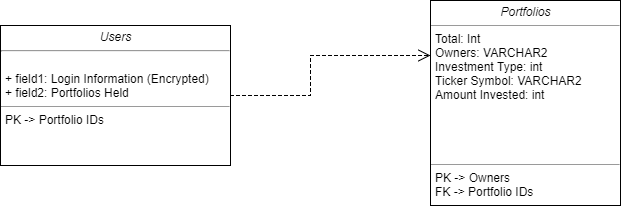
\includegraphics[width=14cm]{database.png}
\caption{UML Database Diagram}
\end{figure}

%Every application, however trivial, uses patterns. Some patterns even include things like committing code every
%line change or using automated testing during releases. 
%\section{Patterns use viewpoint}
%Our application will be very intuitive in design which means that we will be using similar patterns in %functionality and design throughout and won't differ heavily. 

\subsection{Design Concerns}

\section{Interface viewpoint}

    Interface viewpoint outlines how three of the core functions interface and interact with one another.
    Beginning with the user interface where portfolio owners can add and remove stocks and options which
    sends updates to the database where the data is stored. The portfolio view also has graphs, charts, histograms,
    and data tables which will be retrieved from various APIs including websites like Quandl and Google Finance.
    
\subsection{Design Elements}
    \begin{itemize}
        \item User Interface
        \item APIs
        \item Database
    \end{itemize}

\subsection{Interface Attributes}

    The user interface is the mobile application that will be used as a front end display for portfolios. Most
    interactions will come from this section, instead of getting called to. Databases will send back information
    regarding account info, portfolio data and ownership, and log in. The web services like Quandl and Google 
    Finance will also send response data to the mobile application which can then process that data into charts 
    and other forms of processable information.

\begin{figure}[h]
\centering
\captionsetup{justification=centering}
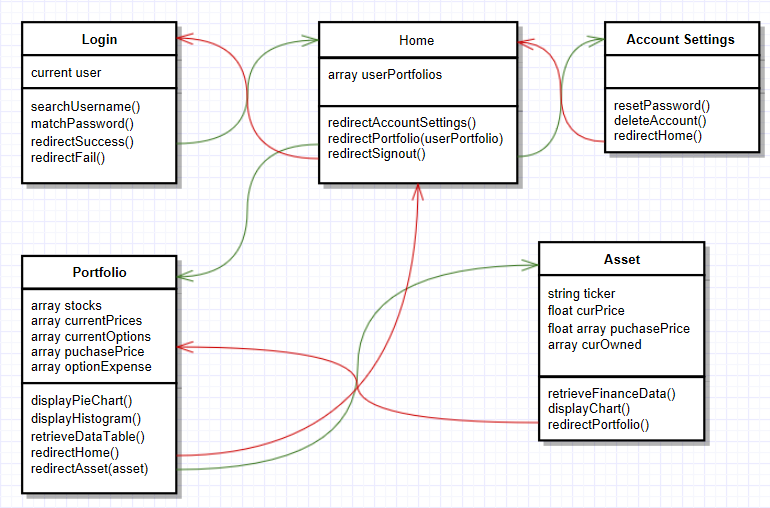
\includegraphics[width=14cm]{frontend.png}
\caption{UML User Interface Diagram}
\end{figure}
    
    The web services and APIs that will be connected to our application will mainly be called from the user
    interface. When a portfolio attempts to display a histogram of stock prices, calls will be made from the user
    interface to a wrapper for Quandl's API. Periodically, the web service will make calls to the APIs and 
    then report this information to the database. This will continually keep our database's information
    up to date which allows for quicker loading on the front end.
    
    The database will be a strong point of interaction in our project. The user interface will interact heavily
    post log in of a user as the application will load all the information on a specific user's portfolios and their
    data. The application will also add or remove information to the database with calls when the user is adding 
    a new stock or option or removing one of the two asset classes. The web services will also be connecting
    to the database periodically to update its information on stock prices or stock splits.
    
    

\end{document}
